\chapter{Interfaccia grafica}
\label{ch:appendice:interfaccia-grafica}

\section*{Legenda}

\subsection*{Risultati di ricerca}
\begin{description}
	\item[$S$] \hfill \\
	Insieme dei risultati di ricerca.
	\item[$S_v$] \hfill \\
	Insieme dei risultati di ricerca visualizzati ($S_v \subseteq S$).
	\item[$s$] \hfill \\
	Rislutato della ricerca ($s \in S$).
\end{description}

\subsection*{Filtri di ricerca}
\begin{description}
	\item[$U$] \hfill \\
	Insieme dei possibili valori di una proprietà ($U = U_A \cup U_B$).
	\item[$U_A \subseteq U$] \hfill \\
	Insieme dei valori autorizzati di una proprietà ($U_A \cap U_B \neq \emptyset$).
	\item[$U_B \subseteq U$] \hfill \\
	Insieme dei valori bloccati di una proprietà ($U_A \cap U_B \neq \emptyset$).
	\item[$u$] \hfill \\
	Valore di una proprietà ($u \in U$).
\end{description}

\subsection*{Cronologia}
\begin{description}
	\item[$r$] \hfill \\
	Ampiezza di ciascuna unità di tempo (espressa in giorni, mesi o anni).
	\item[$t$] \hfill \\
	Numero delle unità di tempo visualizzate.
	\item[$c$] \hfill \\
	Numero massimo di contenuti visualizzati in ciascuna unità di tempo $t_i$.
	\item[$t_i$] \hfill \\
	Unità di tempo i-esima.
	\item[$c_i$] \hfill \\
	Numero di risultati di ricerca associati all'unità di tempo $t_i$.
\end{description}

\section*{Diagrammi dei casi d'uso}

\begin{figure}[ht]
	\begin{center}
    	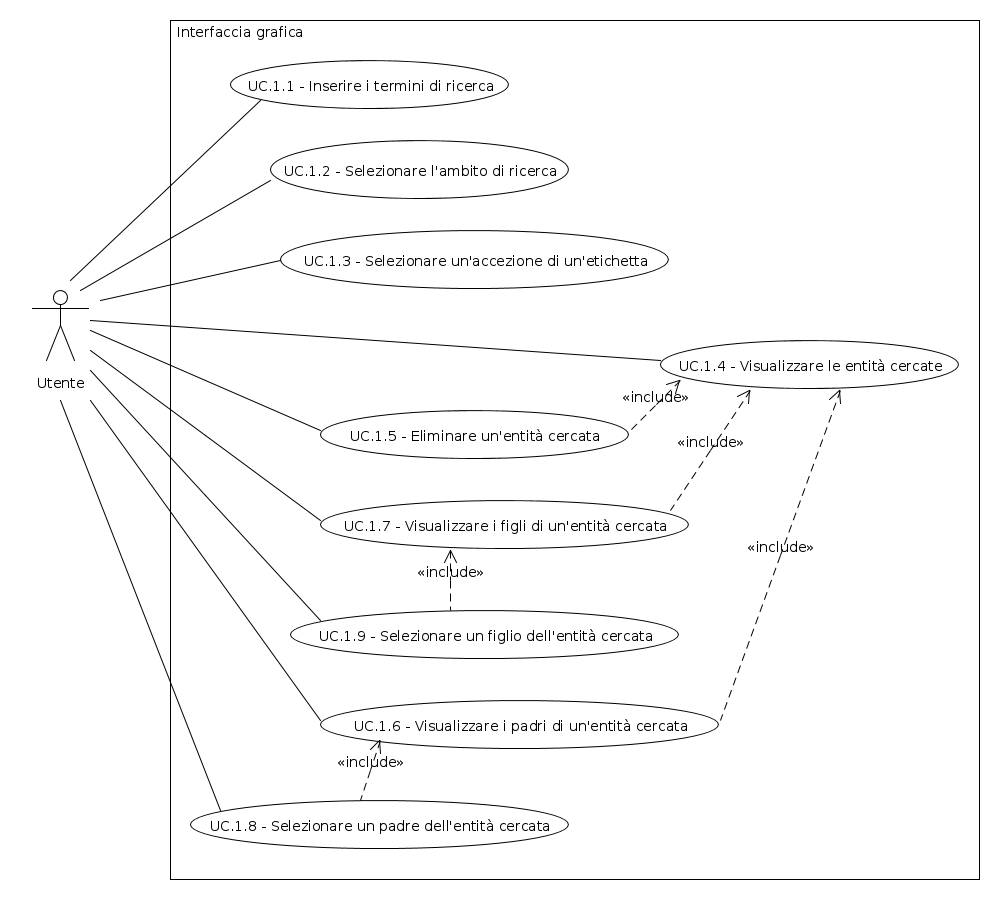
\includegraphics[width=12cm]{img/uc_1.png}
		\label{gfx:uc:1}
		\caption{UC.1 - Ricerca di contenuti informativi}
	\end{center}
\end{figure}

\begin{figure}[ht]
	\begin{center}
    	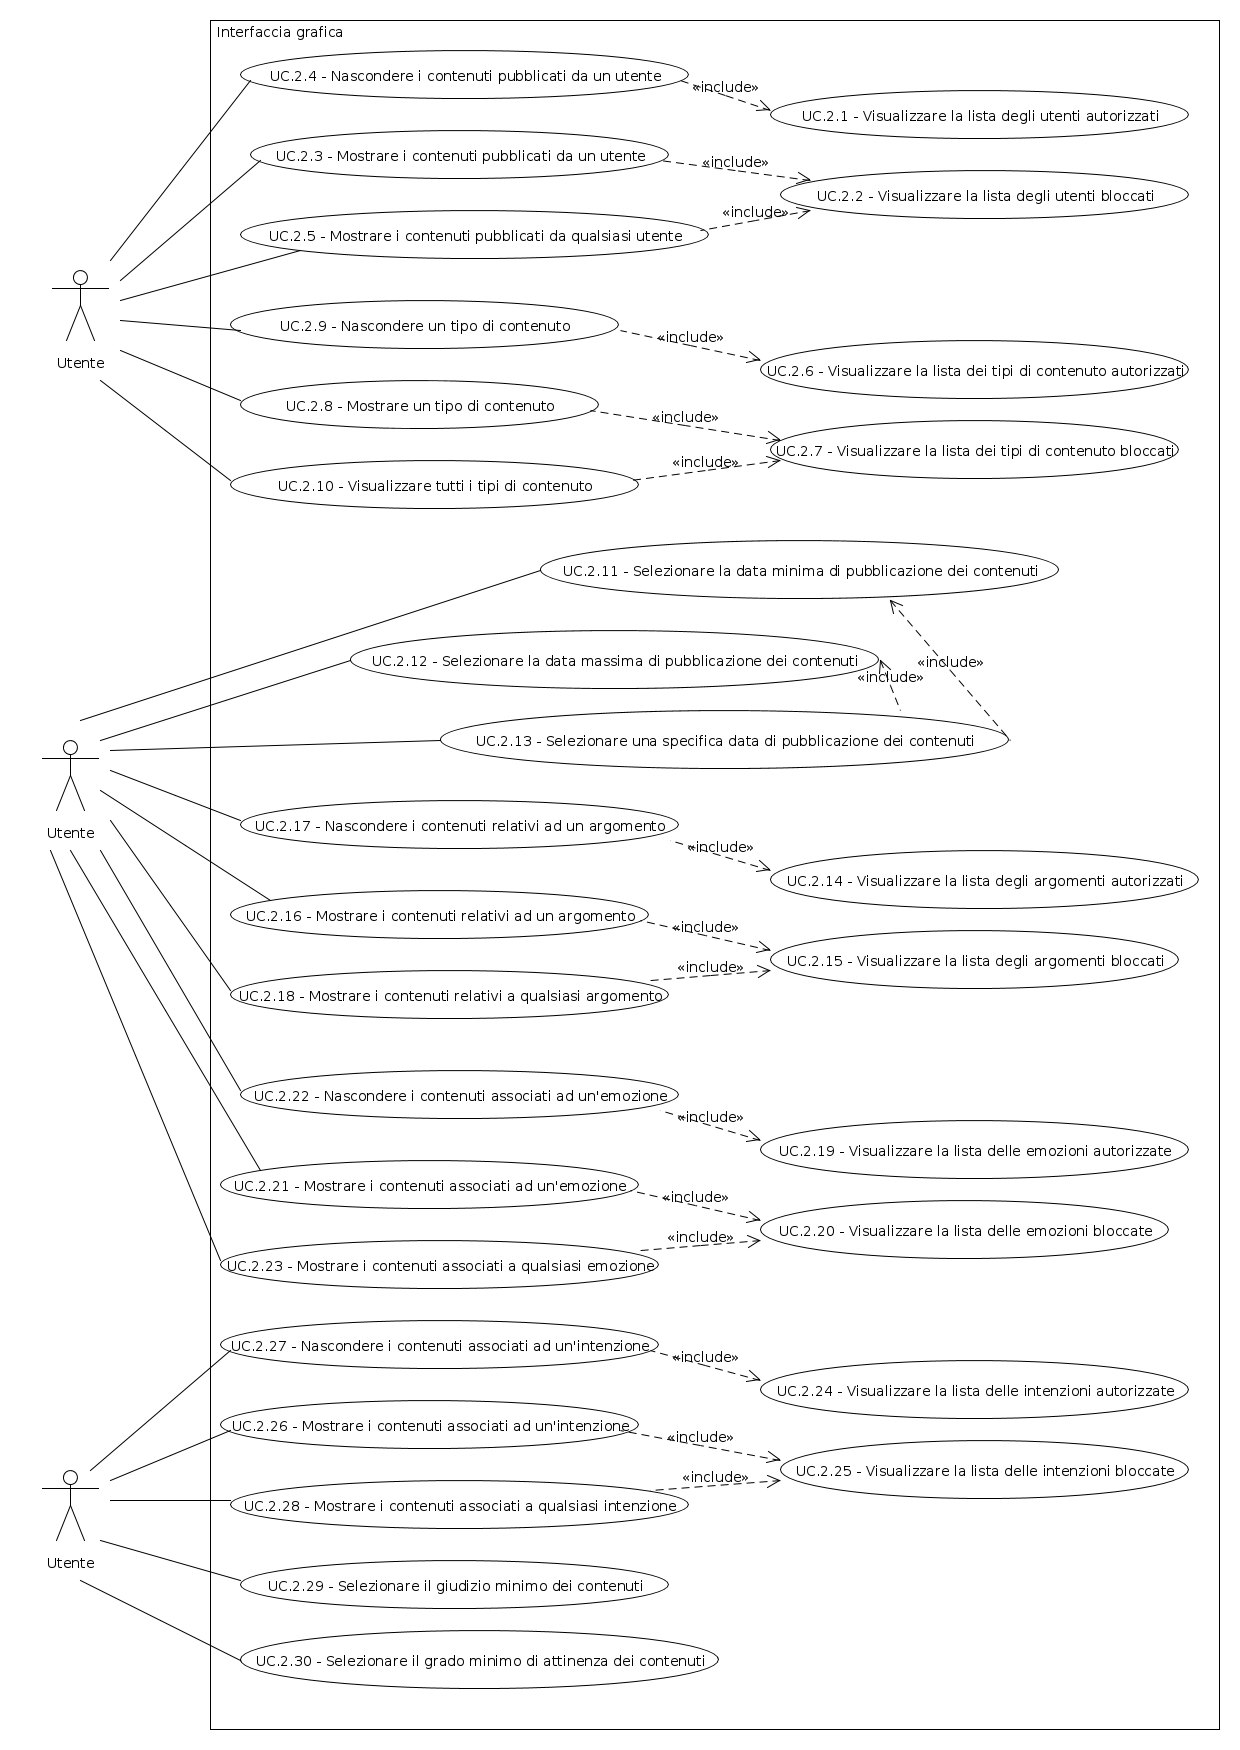
\includegraphics[width=12cm]{img/uc_2.png}
		\label{gfx:uc:2}
		\caption{UC.2 - Raffinamento dei criteri di ricerca}
	\end{center}
\end{figure}

\begin{figure}[ht]
	\begin{center}
    	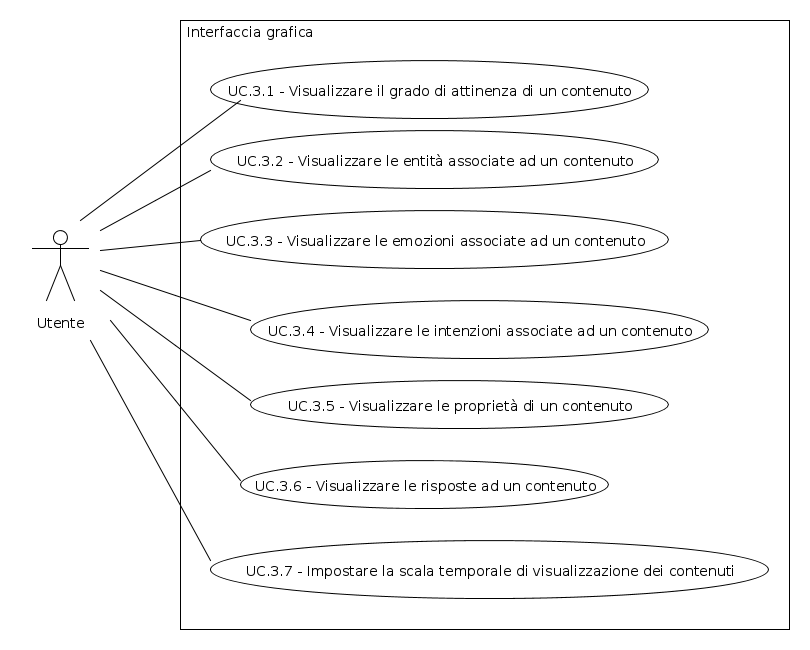
\includegraphics[width=12cm]{img/uc_3.png}
		\label{gfx:uc:3}
		\caption{UC.3 - Consultazione dei risultati di ricerca}
	\end{center}
\end{figure}

\begin{figure}[ht]
	\begin{center}
    	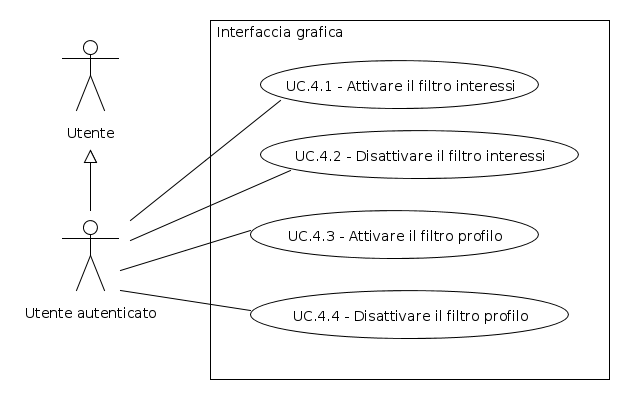
\includegraphics[width=12cm]{img/uc_4.png}
		\label{gfx:uc:4}
		\caption{UC.4 - Gestione dei filtri utente}
	\end{center}
\end{figure}
